
\documentclass[
    oneside,
    fontsize=10pt,leqno]{article}
\usepackage[utf8x]{inputenc}
\usepackage[T1]{fontenc}
\usepackage[english]{babel}
\usepackage{enumitem}
\usepackage{amsfonts,amssymb,amsmath,amsthm}
\usepackage{graphicx}
\usepackage{float}
\usepackage{multirow}
\usepackage{booktabs}
\usepackage{mathtools}
\usepackage{mathptmx} % Times Roman
\usepackage{microtype} % improved character rendering
\usepackage{natbib}
\bibliographystyle{plainnat}


\graphicspath{{./figures/}}

\newtheorem{assumption}{Assumption}
\newtheorem{prop}{Proposition}
\newtheorem{corollary}{Corollary}
\newtheorem{remark}{Remark}


\begin{document}
\title{Participation Costs, Social Capital, and the Limits of Mobility Policy\\[4pt]
{\normalsize\itshape A Model of Status Competition under Income Inequality}}
\author{Anurag Srivastava\\
  \small Riskcare Ltd.\\
  \small Email: anurag.srivastava@riskcare.com \quad ORCiD: 0000-0002-6477-4430\\
  \small \textit{Corresponding author}}
\maketitle

\begin{abstract}
Status-related expenditure rises with income inequality, contrary to
post-war predictions. We show that this empirical regularity is the
generic equilibrium outcome once participation in status competitions
is treated as an endogenous, income-constrained decision. In the
model, a single high-income participant competes against $Q$
low-income participants through tournaments combining innate ability
and acquired social capital, where social capital requires a
threshold expenditure. Under diminishing wealth utility, only two
stable Nash equilibria exist: universal participation and elite-only
participation. A closed-form participation threshold identifies the
joint configuration of income differences and participation costs
that sustains each equilibrium, and reveals why higher inequality
and higher status expenditure can coexist: wider income gaps
simultaneously strengthen the high-income participant's investment
incentive and price out low-income challengers. For policy, two
implications follow. First, reducing participation costs and raising
the meritocratic weight on raw talent are complements, not
substitutes: neither instrument alone can raise class-level mobility
above a hard ceiling of $\mu/[2(1-\mu)]$, where $\mu$ is the
talent weight --- the weight on raw ability relative to social capital. Second, this ceiling
is the binding constraint precisely in the empirically relevant
regime --- large competitions with many challengers --- where both
the equilibrium and collective mobility converge to it
simultaneously. We characterise the precise conditions under which a
third equilibrium, in which only low-income participants invest,
emerges and collapses as competition size grows.

\medskip
\noindent\textbf{Keywords:} status competition; income inequality; social capital;
participation threshold; mobility ceiling; public policy

\medskip
\noindent\textbf{JEL classification:} D31, J62, Z13

\end{abstract}


\section{Introduction}

\noindent

Whether income inequality intensifies or dampens competition for
social position is an old question with a surprisingly durable
empirical answer. Post-war scholars --- Hirsch
(\citeyear{HirschSocialLimits}), Galbraith
(\citeyear{GalbraithAffluent}), and Frank (\citeyear{FrankPond})
--- predicted that rising living standards and narrowing income gaps
would intensify positional rivalry, as more participants could
afford to compete for a fixed stock of social rank. Contemporary
evidence consistently finds the opposite: status-related expenditure
rises with inequality rather than falling with it, with education
expenditure in China \citep{JinLiWu2011} or conspicuous goods across multiple countries
\citep{ChaiKausKiedaisch2019, JaikumarConspConIneq} providing systematic documentation.

This paper concerns itself with the specific form of status
expenditure that has direct consequences for economic outcomes:
investment in educational credentials and institutional affiliation.
Credentials are positional goods in the sense of
\citet{HirschSocialLimits}: their competitive value derives from
the scarcity of the positions they unlock, not solely from the
human capital they embody. In Bourdieu's framework \citep{Bourdieu1977,Bourdieu1986}, credentials function as institutionalised cultural capital: they confer competitive advantage in selection processes through the social recognition they command rather than solely through the productivity they embody. Rising inequality raises both the stakes of winning a
credentialled position and the structural advantage of those who can
afford the threshold investment required to compete --- which is why
education expenditure and inequality may move together in the data. The
present model treats education as such a credential rather than as
a productive asset that accumulates individual capacity across jobs.
This focus reflects the observed reality that access to economic
goods --- elite occupations, professional status, income at the top
of the distribution --- is often allocated through positional
competition rather than anonymous market clearing
\citep{Rivera2015Pedigree, LaurisonFriedman2016, Bourdieu1986}:
credentialism is the mechanism, not an aberration from it.

The source of the discrepancy, we argue, lies in a common
simplification: existing models of status competition treat the
participation decision as a continuous intensity choice --- agents
decide how much to invest in status-enhancing social capital, with
income affecting the level of investment but not whether entry is
feasible at all. A threshold cost structure that makes
participation a discrete binary decision --- affordable or not,
depending on income --- allows us to inspect the effects of income inequality on binary outcomes of success and shows that wider income gaps simultaneously strengthen the
high-income participant's investment incentive and price out
low-income challengers. The positive association between inequality
and status expenditure follows as the generic equilibrium outcome, not a special case.

The model's specific architecture --- the separation of talent
$\mu r_i$ from social capital $(1-\mu)s_i$ as distinct components
of competitive rank --- is motivated by several empirical patterns
in the elite mobility literature that the standard Becker-Tomes
human capital framework doesn't generate without
auxiliary assumptions about non-productive forms of capital.
\citet{LoBelloMorchio2022} find that dynastic workers in the UK
who follow their parent's occupation find jobs faster but earn
\emph{lower} wages than comparably qualified non-dynastic workers;
human capital theory predicts wage parity or a premium, not a
penalty. \citet{LaurisonFriedman2016} show that the class-origin
pay gap in British elite occupations varies sharply by occupation
type: it is close to zero in science, academia, and the built
environment but approximately 20\% in finance, law, and
accountancy --- the opposite of a human capital view since 
the gap should be largest where inherited knowledge is most
valuable. The data are directly consistent with the model's
prediction that the class gap is increasing in $(1-\mu)$, the
social capital weight: finance and law are low-$\mu$ occupations
where networks and cultural fit dominate, while science and
engineering are high-$\mu$ occupations where technical output is
directly measurable. \citet{MockettiRomaRubolino2022} exploit two waves of liberalisation of professional services in Italy and find that deregulation reduces intergenerational occupational persistence, with the effect concentrated among less able dynastic workers (proxied by delayed school qualification) --- consistent with the model's prediction that social capital weight $(1-\mu)$ determines how far raw talent shortfalls can be compensated by positional advantages, so that low-$r_i$ incumbents are the first to exit when regulatory protection shrinks.
\footnote{A related finding concerns
UK university admissions, where personal statements --- a threshold
social capital investment requiring coaching and institutional
support --- have negligible predictive validity for university
performance \citep{JonesSuttonTrust2013}, and students from less
advantaged backgrounds out-perform peers from more advantaged
backgrounds with the same entry grades. This is consistent with
the model's architecture but pertains specifically to education
admissions rather than labour market competition.} These residuals
share a common structure: each identifies a component of elite
access that facilitates entry without raising productivity, and
whose weight varies across occupations. That component is the
social capital weight $(1-\mu)$ in the present model.

Against this backdrop, the paper develops the following model.
The model considers a status competition in which one
high-income participant competes against $Q \geq 1$ low-income
participants through a probabilistic tournament combining innate
ability and acquired social capital. Social capital --- the skills,
credentials, and network affiliations that institutional engagement
provides --- can be obtained only by paying a threshold cost
$\overline{\nu}$, making it accessible to the high-income
participant by default and contingent on budget feasibility for
low-income participants. The probability of advancement depends on
both components, with social capital weighted more heavily than raw
talent, following the empirical literature on elite hiring
\citep{Rivera2015Pedigree, Bills2003Credentials}. Status enters
utility indirectly through its effect on future income, following
\citet{postlewaite1998socialbasisinterdeppreferences}; no separate
taste for rank is required.

The model yields four results with direct policy content.
First, under diminishing wealth utility only two stable
Nash equilibria exist: universal participation (both invest) and
elite-only participation (only the high-income participant invests).
The transition between them is governed by a participation threshold
$\overline{\nu}^{*}$ that decreases in both competition size $Q$
and the social capital weight $(1-\mu)$. Wider inequality sustains
high-income investment even as it prices out low-income
challengers, which is why status expenditure and inequality rise
together.

Second, collective low-income mobility converges to a hard ceiling
of $\mu/[2(1-\mu)]$ in the empirically relevant regime. This
ceiling is bounded strictly below one-half for all admissible
$\mu$, and falls as social capital is weighted more heavily. It
represents a structural limit that no participation-boosting policy
can overcome without also raising $\mu$. Reducing participation
costs alone expands the range of inequality levels consistent with
universal participation, but the ceiling itself is determined by
the design of the competition, not the number of participants.

Third, these two instruments are complements in a precise sense: the
participation threshold $\overline{\nu}^{*}$ is increasing in $A$,
a composite parameter embedding both $Q$ and $\mu$, and the ceiling
$\mu/[2(1-\mu)]$ is increasing in $\mu$. Policies that lower
$\overline{\nu}$ (credential subsidies, open-access qualifications,
reduced network barriers) shift the equilibrium toward universal
participation; policies that raise $\mu$ (standardised assessment,
transparent merit criteria) raise the ceiling at which collective
mobility converges. Neither alone is sufficient.

Fourth, a third equilibrium --- in which only low-income
participants invest while the high-income participant free-rides on
raw talent --- requires reference-dependent preferences inverting
the standard concavity ordering, and is viable only in small
competitions ($Q = 1$ or $2$). This provides a formal account of
the over-investment in elite credentials observed among aspiring
candidates from lower-income backgrounds in narrow selection
processes \citep{Rivera2015Pedigree}: the mechanism
is both preference-dependent and competition-size-specific, and
cannot survive scaling to large standardised assessments.

These results position the paper relative to its quantitative
predecessors as follows. The two closest --- each reaching conclusions
that diverge from the present paper --- fix the participant pool.
\citet{FrankAER1984} shows that wider wage dispersion reduces
competition intensity --- workers accept wage penalties to occupy
the top of the local rank distribution, so narrowing inequality
intensifies rivalry. \citet{ColeMailaithPostlewaite1992} derive
status concern from the marriage market and show directly that
agents from a more compact income distribution save more, again
implying that narrowing inequality raises status expenditure. In
both cases income distribution shapes the intensity of competition
within the participant pool, but participation itself is not
subject to a threshold budget constraint --- all agents compete,
and the question is how intensely. Both models therefore predict
that \emph{narrowing} inequality raises status expenditure, the
opposite of the empirical finding. The present paper introduces a
threshold participation cost that makes entry a discrete binary
decision, and shows that this single change reverses the sign:
\emph{widening} inequality raises status expenditure by sustaining
high-income investment while pricing out low-income challengers.

The most directly comparable model is that of
\citet{GalliceGrillo2019}, who consider a model in which
educational investment entails productivity gains, signaling power,
and social status simultaneously, with status depending on relative
achievement in one of three dimensions: innate skills, level of
schooling, and income. They characterise conditions under which
social concerns increase or decrease educational and income
inequality. The present paper asks a different question: not how much agents invest
conditional on universal participation, but whether participation
itself is feasible across income levels. The current paper generates a structural bound and allows hierarchy-related conclusions for mobility using the ceiling $\mu/[2(1-\mu)]$ and the binary equilibrium classification (EP--FP) which arise specifically from the threshold cost structure and income asymmetry -- claims that don't follow from the Gallice and Grillo model -- where all agents participate with varying investment intensity. Whether inequality amplifies or
dampens status investment conditional on universal participation is
a distinct question from whether inequality sustains or destroys
participation itself.

The threshold cost structure used in the paper is motivated by broader literature on social capital and credential investment \citep{Jencks1979, HeckmanMosso2014}. Participation costs in elite competitions --- tuition fees, membership dues, network cultivation
--- are threshold rather than continuous expenditures: they must be
paid in full to unlock the social capital they confer. This
threshold structure is central to the model's ability to generate
binary equilibrium outcomes and a closed-form participation
condition. The sociological literature \citep{wegener1992prestigeconcepts,
MijsParadox2021, MijsMeritocracy2020} motivates the empirical
puzzle and the inclusive-participation (IP) over-investment result, but the model does
not require the sociological apparatus: all results follow from
standard expected-utility maximisation with a threshold entry cost.

The paper proceeds as follows.
Section~\ref{sec:Theoretical_chapter_Model} develops the model,
deriving winning probabilities for all four investment cases under
general $Q$, characterising the Nash equilibria, deriving the
participation threshold in closed form, and establishing the
mobility ceilings. Section~\ref{sec:Policy} draws out the policy
implications, mapping the model's parameters onto observable
competition structures. Section~\ref{sec:Conclusion} concludes.

\section{\label{sec:Theoretical_chapter_Model}Model}

\subsection{Basic Setup}

\noindent

We consider a status competition in which a single high-income participant competes against $Q\geq1$ low-income participants ($Q+1$ total).
The high-income participant occupies the high-income position $y_{2}$ and
seeks to maintain it; each low-income participant receives income $y_{1}<y_{2}$
and seeks promotion. Two characteristics determine performance in
the competition. First, \emph{raw talent} $r_{i}\sim\mathrm{Uniform}[0,1]$,
which cannot be affected by expenditure. Second, \emph{social capital}
$s_{i}\sim\mathrm{Uniform}[0,1]$, which can be enhanced only by paying
a threshold cost $\overline{\nu}$. Both $r_{i}$ and $s_{i}$ are
independently distributed and unknown to participant $i$ before the
competition. The participant with the highest composite score $\mu
r_{i}+(1-\mu)s_{i}$ wins the high-income position, where $\mu\in(0,1)$
weights raw talent relative to social capital.

Since all $Q$ low-income participants share the same income $y_{1}$ and
all face the same investment decision, we analyze the participation
problem from the perspective of a representative low-income participant.
The high-income participant's decision is analogous. A participant pays
$\overline{\nu}$ to access social capital (setting $s_{i}>0$) or
abstains and saves instead (setting $s_{i}=0$, relying on raw talent
alone). Crucially, no participant knows $r_{i}$ or $s_{i}$ prior
to deciding whether to pay $\overline{\nu}$, so investment decisions
depend only on the income class of the participant.

Status enters utility only indirectly: the winner obtains disposable
income $y_{2}$ in the following period, the loser retains $y_{1}$.
This treatment, following \citet{postlewaite1998socialbasisinterdeppreferences},
preserves a standard wealth-utility framework while endogenising the
social dimension of the competition.

The model is designed for a specific class of competitions: those
in which a fixed number of high-income positions is contested by a
variable pool of challengers, and in which the winner's gain is
the loser's foregone advancement. This zero-sum structure is not
a simplifying approximation but an accurate description of
positional competitions for elite credentials --- partnership
tracks at professional firms, senior academic appointments,
competitive university admissions --- where the number of positions
is institutionally fixed and occupying one precludes others from
doing so. The model does not speak to general labour markets in
which education raises productivity across all jobs, nor to settings
in which a losing investor retains a human capital gain from the
investment. That class of questions --- where social capital raises
$y_1$ as well as the probability of winning $y_2$ --- is a natural
extension in which the threshold cost generates a productivity
externality for non-winners; we leave it to future work. The
present model isolates the participation and mobility effects of
threshold costs in positional competitions, which is the mechanism
most directly relevant to the empirical puzzle that motivates it.

Focusing on conditions where the contest advantage from social capital
investment is substantial, we assume
throughout that social capital is weighted more heavily than raw talent:

\begin{assumption}
\label{assu:mu_less_than_half}$\mu<\frac{1}{2}$
\end{assumption}

\noindent\textbf{Remark on distributional assumptions.}
The uniform distributions for $r_i$ and $s_i$ are adopted for
tractability: they yield the closed-form trapezoidal CDF
$F_X(x)$ whose piecewise structure drives the winning probability
derivations in Appendix~\ref{sec:appendix_theoretical_1}. The
key qualitative results do not depend on uniformity. The
fundamental ordering $p_1 < 1/(Q+1) < p_1'$ --- which drives the
Nash equilibrium analysis --- holds for any pair of distributions
that are symmetric on $[0,1]$ and have the same marginal
distribution for $r_i$ and $s_i$, since the ordering follows from
the structural disadvantage of competing without social capital
against an opponent who has it, not from the specific shape of the
distributions. The closed-form expressions for $p_1$, the
participation threshold $\overline{\nu}^*$, and the mobility
ceiling $\mu/[2(1-\mu)]$ are specific to the uniform case, but
the existence of the binary equilibrium structure (exclusive participation, EP, and~full participation, FP,
as the only generically stable equilibria under diminishing
utility), and all comparative statics on $Q$, $\mu$, $\overline{\nu}$,
and $y_2 - y_1$ extend to the broader distributional class. The
uniform specification thus functions as a parametric
representation of a more general result rather than a special
case on which the argument depends.

\medskip
\noindent The distribution of the composite score $x_{i}\equiv\mu
r_{i}+(1-\mu)s_{i}$ under Assumption~\ref{assu:mu_less_than_half}
is trapezoidal (derived in Appendix~\ref{sec:appendix_theoretical_1}),
with CDF $F_{X}(x)$ that is piecewise quadratic on $[0,\mu]$, linear
on $[\mu,1-\mu]$, and piecewise quadratic on $[1-\mu,1]$.

The four investment cases are as follows.

\begin{itemize}
\item \textbf{Exclusive Participation (EP)} --- High-income invests ($\nu_{2}=\overline{\nu}$), low-income
do not ($\nu_{1}=0$).
\item \textbf{Inclusive Participation (IP)} --- Low-income invest ($\nu_{1}=\overline{\nu}$), high-income
does not ($\nu_{2}=0$).
\item \textbf{Full Withdrawal (FW)} --- Neither invests ($\nu_{1}=\nu_{2}=0$).
\item \textbf{Full Participation (FP)} --- Both invest ($\nu_{1}=\nu_{2}=\overline{\nu}$).
\end{itemize}

\subsection{\label{subsec:Two-player-Discrete-Model}Equilibrium Conditions}

\noindent

\subsubsection{Winning Probabilities}

The derivations are in Appendices~\ref{sec:appendix_theoretical_1}
and~\ref{sec:appendix_theoretical_2}. The per-low-income-participant
winning probabilities are:

\begin{align}
p_{1} & =\frac{\mu}{2(1-\mu)(Q+2)} & & \text{(EP)}\label{eq:p1_caseI}\\[4pt]
p_{1}' & =\frac{6-7\mu}{6(1-\mu)} & & \text{(IP, }Q=1\text{)}\label{eq:p1prime_Q1}\\[4pt]
p_{1} & =\frac{1}{Q+1} & & \text{(FW and FP)}\label{eq:p_baseline}
\end{align}

In EP, the low-income participant competes on raw talent alone
against the high-income participant's full composite score --- a
structural disadvantage that drives $p_{1}$ strictly below the
symmetric baseline $1/(Q+1)$. In IP the roles are reversed:
the investing low-income participant has the full score advantage,
pushing $p_{1}'$ strictly above the baseline. For FW and FP,
symmetry gives $1/(Q+1)$ directly. For general $Q\geq2$, $p_{1}'$
is computable as a rational function of $\mu$ of degree $Q$
(Appendix~\ref{sec:appendix_theoretical_2}); all equilibrium
results for IP follow from the ordering result alone, without
requiring a closed form for $p_{1}'$.

The high-income participant's probability follows from $p_{2}=1-Q\,p_{1}$
in each case.

\medskip

The fundamental ordering that drives the Nash equilibrium analysis
follows directly from Assumption~\ref{assu:mu_less_than_half}:

\begin{gather}
p_{1}<\frac{1}{Q+1}<p_{1}'\quad\text{for all }Q\geq1,\;\mu<\tfrac{1}{2}\label{eq:ordering}
\end{gather}

Figure~\ref{fig:Probability-of-winning} illustrates these probabilities.
Panel (a) shows that $p_{1}$ (EP) lies strictly below the baseline
$1/(Q+1)$ and decays rapidly with $Q$. Panel (b) shows $p_{2}$
(EP, high-income participant) lying well above the baseline. Panel (c)
shows $p_{1}'$ (IP, $Q=1$) strictly above the baseline throughout.
Panel (d) is discussed in Section~\ref{subsec:Mobility-Ceiling}.

\begin{figure}[H]
\begin{centering}
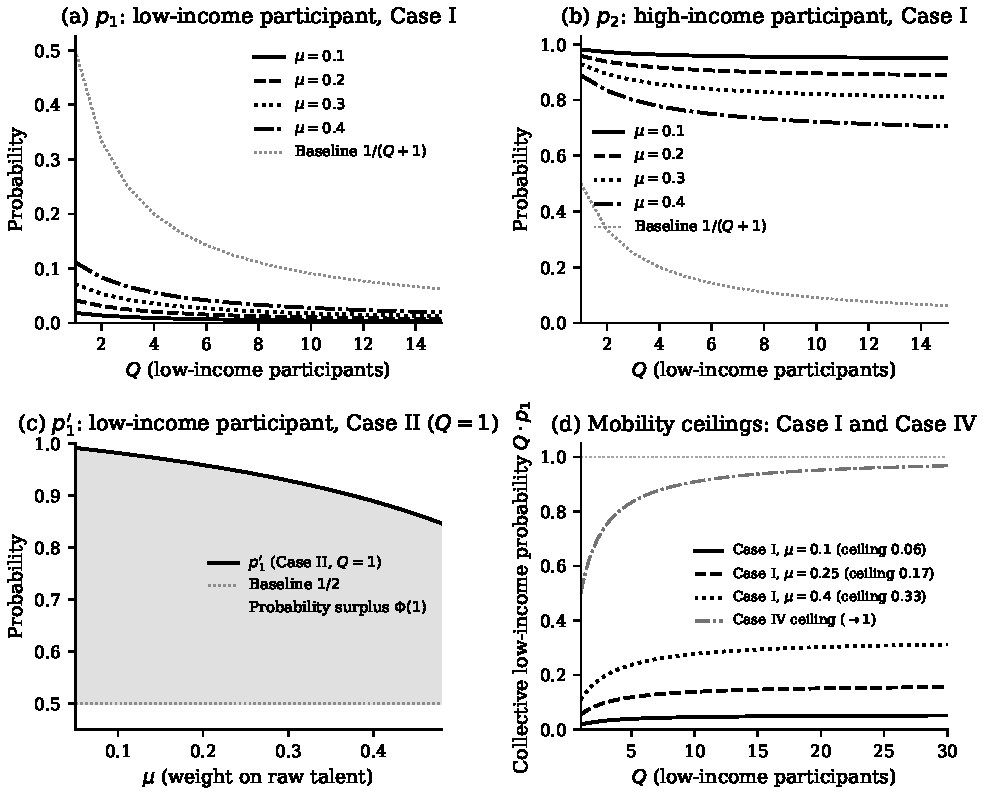
\includegraphics[width=\textwidth]{winprob_main}
\par\end{centering}
\caption{\label{fig:Probability-of-winning}Winning probabilities and mobility
ceiling. One high-income participant, $Q$ low-income participants. Dotted horizontal
lines in panels (a)--(b) show baselines $1/(Q+1)$ for each $Q$.}
\end{figure}

\subsubsection{Intertemporal Choice and Utility Payoffs}

Participants optimise an intertemporally additive utility $u(\cdot)$
over $T$ periods. In period 1 each participant decides whether to
pay $\overline{\nu}$; from period 2 onward she receives the income
corresponding to her position. Define the $T$-period discount sum
$D_{T}=\sum_{t=0}^{T-2}\delta^{-t}=(1-\delta^{-(T-1)})/(1-\delta^{-1})$,
where $\delta>1$ is the discount factor. The case $T=2$ gives $D_{T}=1$
and recovers the standard two-period model. The expected lifetime
utilities are:

\begin{align*}
\text{Low-income participant:} & \quad u(y_{1}-\nu_{1})+\frac{D_{T}}{\delta}\bigl[p_{1}^{c}\,u(y_{2})+(1-p_{1}^{c})\,u(y_{1})\bigr]\\
\text{High-income participant:} & \quad u(y_{2}-\nu_{2})+\frac{D_{T}}{\delta}\bigl[p_{2}^{c}\,u(y_{2})+(1-p_{2}^{c})\,u(y_{1})\bigr]
\end{align*}

where $p_{i}^{c}$ denotes the winning probability in case $c\in\{\mathrm{EP,IP,FW,FP}\}$.
Define the utility costs of participation:

\begin{align*}
U_{1}\equiv u(y_{1})-u(y_{1}-\overline{\nu}),\qquad U_{2}\equiv u(y_{2})-u(y_{2}-\overline{\nu})
\end{align*}

Under diminishing marginal utility with $y_{1}<y_{2}$: $U_{2}<U_{1}$.
Table~\ref{tab:prisoners_dilemma_cases} summarises the four cases
as a $2\times2$ game; full utility payoffs are in
Table~\ref{tab:prisoners_dilemma} (Appendix~\ref{sec:appendix_payoffs}).

\begin{table}[H]
\centering
\caption{\label{tab:prisoners_dilemma_cases}Investment strategies}
\smallskip
\begin{tabular}{lcc}
\toprule
 & \textit{Low-income withdraws} & \textit{Low-income invests}\\
\midrule
\textit{High-income withdraws} & FW        & IP\\
\textit{High-income invests}   & EP        & FP\\
\bottomrule
\end{tabular}
\end{table}


The full utility payoffs for each case are reported in
Table~\ref{tab:prisoners_dilemma} in Appendix~\ref{sec:appendix_payoffs};
the equilibrium conditions below are derived from those payoffs.

\subsubsection{\label{subsec:Nash-Equilibrium-Conditions}Nash Equilibrium Conditions}

For ease of notation define the probability-gap terms:

\begin{gather}
p_{1}\equiv\frac{\mu}{2(1-\mu)(Q+2)},\quad p_{2}\equiv1-Q\,p_{1}\nonumber\\
p_{1}'\equiv\frac{6-7\mu}{6(1-\mu)}\;(Q=1)\label{eq:probabilities}
\end{gather}

The ordering $p_{1}<1/(Q+1)<p_{2}$ and $p_{1}'>1/(Q+1)$
holds for all $\mu<1/2$ (Equation~\ref{eq:ordering}). Note that
$p_{2}'=1-Q\,p_{1}'$ satisfies $p_{2}'<1/(Q+1)$ by the same
ordering, but $p_{2}'$ does not appear in the equilibrium conditions
below: by the algebraic identity $1/(Q+1)-p_{2}'=Q(p_{1}'-1/(Q+1))$,
it is replaced throughout by $Q\cdot\Phi(Q)$, which is valid for all
$Q\geq1$. We define $\Phi(Q)$ now, before analysing the cases, since
it appears in both EP and IP:

\medskip
\noindent The \emph{probability surplus} $\Phi(Q)$ is the gain in
winning probability a low-income participant obtains from being the
sole investor in social capital relative to the symmetric
no-investment baseline, scaled by the utility gap and discount
factor:
\begin{align}
\Phi(Q) & \equiv\frac{D_{T}}{\delta}\left(p_{1}'-\frac{1}{Q+1}\right)(u(y_{2})-u(y_{1}))\label{eq:Phi_def}
\end{align}

\noindent Since $p_{1}'>1/(Q+1)$ for all $\mu<1/2$
(Equation~\ref{eq:ordering}), $\Phi(Q)>0$ always. For $Q=1$,
substituting $p_{1}'=(6-7\mu)/[6(1-\mu)]$ yields:
\begin{align}
\Phi(1) & =\frac{D_{T}}{\delta}\cdot\frac{3-4\mu}{6(1-\mu)}\cdot(u(y_{2})-u(y_{1}))\label{eq:Phi_Q1}
\end{align}

\noindent where $(3-4\mu)>0$ under Assumption~\ref{assu:mu_less_than_half},
so $\Phi(1)$ is strictly positive and decreasing in $\mu$, ranging
from $\Phi(1)\to1/2$ at $\mu\to0$ to $\Phi(1)\to1/3$ at $\mu\to1/2$.
By Proposition~\ref{prop:asymptotic_phi} below, $\Phi(Q)\sim1/[Q(Q+1)]$
asymptotically, so the surplus narrows rapidly with competition size.

\medskip
\noindent\textbf{Exclusive Participation (EP)} (high-income invests, low-income withdraws) is a Nash
equilibrium if and only if:\footnote{Derived from the payoff table (Appendix~\ref{sec:appendix_payoffs}): the low-income participant prefers not to invest, and the high-income participant prefers to invest, given the other\'s strategy.}

\begin{gather}
\frac{D_{T}}{\delta}\left(\frac{1}{Q+1}-p_{1}\right)(u(y_{2})-u(y_{1}))<U_{1}\label{eq:caseI_poor}\\
U_{2}<\frac{D_{T}}{\delta}\left(p_{2}-\frac{1}{Q+1}\right)(u(y_{2})-u(y_{1}))\label{eq:caseI_rich}
\end{gather}

Both conditions hold simultaneously under diminishing utility since
$U_{2}<U_{1}$ and $p_{2}-1/(Q+1)\geq1/(Q+1)-p_{1}$. A higher
$\overline{\nu}$ favors EP so long as the high-income participant retains an incentive
to invest; a lower $\overline{\nu}$ can destabilize it if low-income
participants are induced to enter. Wider income differences ($y_{2}-y_{1}$
larger) reinforce the high-income participant's incentive to invest while
simultaneously raising the stakes enough to attract low-income investment,
making the first condition harder to satisfy.

\medskip
\noindent\textbf{Inclusive Participation (IP)} (low-income invest, high-income withdraws). We now
state this case as a formal proposition, since it requires conditions
beyond standard diminishing utility and its characterisation carries
independent theoretical content. The governing object is $\Phi(Q)$,
defined above. The probability surplus narrows at rate $Q^{-2}$: at
$Q=1$ the IP window is wide ($\Phi(1)\approx0.46$ at $\mu=0.2$),
but by $Q=3$ it has collapsed to $\Phi(3)\approx0.08$ --- an 82\%
reduction --- and by $Q=5$ to $\Phi(5)\approx0.03$
(Table~\ref{tab:phi_values}). The qualitative conclusions of
Proposition~\ref{prop:caseII} --- that IP requires
reference-dependent preferences and that the feasibility window
$[U_1, U_2/Q]$ narrows as $\mu$ increases --- hold for general
$Q\geq1$ by the ordering result in Equation~\ref{eq:ordering}.

\begin{prop}[IP Nash Equilibrium]\label{prop:caseII}
IP (low-income invest, high-income withdraws) is a Nash equilibrium if and
only if:
\begin{gather}
U_{1}<\Phi(Q)\leq U_{2}/Q\label{eq:caseII_NSC}
\end{gather}
A necessary condition is therefore $Q\cdot U_{1}<U_{2}$. Under
standard diminishing utility with $y_{1}<y_{2}$, $U_{2}<U_{1}$,
so $U_{2}/Q<U_{1}$ for all $Q\geq1$ and Condition~\eqref{eq:caseII_NSC}
cannot be satisfied. IP requires reference-dependent preferences
under which $U_{1}<U_{2}$ --- the marginal utility cost of $\overline{\nu}$
is higher for the low-income participant than for the high-income participant, reversing the
standard concavity ordering. For $Q=1$, the condition reduces to:
\begin{align}
U_{1}<\Phi(1)\leq U_{2}\label{eq:caseII_Q1}
\end{align}
which is feasible if and only if $U_{1}<U_{2}$. For general $Q$,
the necessary condition $Q\cdot U_{1}<U_{2}$ tightens as $Q$ grows;
by Proposition~\ref{prop:asymptotic_phi}, $\Phi(Q)\sim1/[Q(Q+1)]$,
so the condition fails for any fixed $U_{1}>0$ beyond
$Q^{*}\approx1/\sqrt{U_{1}}$.
\end{prop}

\begin{proof}
Condition~\eqref{eq:caseII_NSC} is derived directly from the utility
payoffs in Table~\ref{tab:prisoners_dilemma} (Appendix~\ref{sec:appendix_payoffs}). The low-income participant
prefers to invest given the high-income participant withdraws if and only if
$U_{1}<\Phi(Q)$. The high-income participant prefers to withdraw given the
low-income participants invest if and only if the gain from deviating to investment,
$\frac{D_{T}}{\delta}(1/(Q+1)-p_{2}')(u(y_{2})-u(y_{1}))=Q\cdot\Phi(Q)$
(using $1/(Q+1)-p_{2}'=Q(p_{1}'-1/(Q+1))$, valid for all $Q\geq1$),
is less than the cost $U_{2}$, i.e. $U_{2}\geq Q\cdot\Phi(Q)$,
equivalently $\Phi(Q)\leq U_{2}/Q$. Both conditions together require
$U_{1}<U_{2}/Q$. Under standard concavity $U_{2}<U_{1}$, so
$U_{2}/Q<U_{1}$ for all $Q\geq1$ and the condition fails. $\square$
\end{proof}

\medskip

Several features of this proposition deserve comment. First,
$\Phi(1)$ is strictly decreasing in $\mu$: as social capital is
weighted more heavily, the probability surplus from being the sole
investor narrows, and the IP window must be correspondingly
tighter to sustain the equilibrium. At $\mu\to0$ (pure raw-talent
competition), $\Phi(1)\to1/2$, giving the widest possible window;
at $\mu\to1/2$ (Assumption~\ref{assu:mu_less_than_half} binding),
$\Phi(1)\to1/3$. Second, the equilibrium remains fragile even when
it exists: higher $\overline{\nu}$, greater impatience ($\delta$
rising), or wider income differences ($y_{2}-y_{1}$ larger) can each
collapse it into FW or FP respectively.
Third, $\Phi(Q)$ narrows at rate $Q^{-2}$ for general $Q$
(Proposition~\ref{prop:asymptotic_phi}), making IP
quantitatively relevant only for small competitions ($Q=1$ or $2$).
This is consistent with the interpretation that IP ---
over-investment by aspiring low-income candidates in socially
embedded competitions --- is a phenomenon of elite selection
processes with narrow fields, not of large-scale standardised
assessments.

\medskip
\noindent\textbf{Full Withdrawal (FW)} (neither invests) is a Nash equilibrium if:\footnote{Both participants prefer withdrawal given the other withdraws.}

\begin{gather*}
U_{1}>\frac{D_{T}}{\delta}\left(p_{1}'-\frac{1}{Q+1}\right)(u(y_{2})-u(y_{1}))\\
U_{2}>\frac{D_{T}}{\delta}\left(p_{2}-\frac{1}{Q+1}\right)(u(y_{2})-u(y_{1}))
\end{gather*}

Since $p_{1}'-1/(Q+1)\leq p_{2}-1/(Q+1)$ and $U_{2}<U_{1}$, the
binding constraint is the second inequality. FW prevails when
participation costs are prohibitively high relative to the income
gain. If there is any net utility from competition, FP is the
likely outcome.

\medskip
\noindent\textbf{Full Participation (FP)} (both invest) is a Nash equilibrium if:\footnote{Both participants prefer investment given the other invests.}

\begin{gather}
U_{1}<\frac{D_{T}}{\delta}\left(\frac{1}{Q+1}-p_{1}\right)(u(y_{2})-u(y_{1}))\label{eq:caseIV_poor}\\
U_{2}<Q\cdot\Phi(Q)\label{eq:caseIV_rich}
\end{gather}

With $U_{2}<U_{1}$, this equilibrium rests on the low-income participant's
incentive: so long as the low-income participant finds the competition
worthwhile, the high-income participant also participates. Note that
Equations~\ref{eq:caseI_poor} and~\ref{eq:caseIV_poor} are exact
complements --- FP obtains precisely where EP fails for
the low-income participant. The high-income participant's condition
$U_{2}<Q\cdot\Phi(Q)$ uses the algebraic identity
$1/(Q+1)-p_{2}'=Q(p_{1}'-1/(Q+1))$, which holds for all $Q\geq1$
and connects FP directly to the probability surplus $\Phi(Q)$
from Proposition~\ref{prop:caseII}: the high-income participant's boundary
between IP and~FP is exactly $Q\cdot\Phi(Q)$.

\medskip

These conditions confirm that under diminishing utility only EP
and~FP are generically stable. For very low $\overline{\nu}$, both
participants invest (FP); for very high $\overline{\nu}$, only
the high-income participant invests (EP); for sufficiently extreme $\overline{\nu}$,
neither invests (FW). IP requires a non-standard utility
structure and remains fragile throughout.

\subsubsection{\label{subsec:Threshold}Participation Threshold}

The boundary between FP and~EP is defined by the critical
cost $\overline{\nu}^{*}$ at which the low-income participant is indifferent
between investing and withdrawing, given the high-income participant invests.
Setting Equation~\ref{eq:caseIV_poor} as an equality:

\begin{align}
u(y_{1})-u(y_{1}-\overline{\nu}^{*}) & =\frac{D_{T}}{\delta}\left(\frac{1}{Q+1}-p_{1}\right)(u(y_{2})-u(y_{1}))\label{eq:threshold_general}
\end{align}

Under log utility $u(y)=\log(y)$, this yields
$\overline{\nu}^{*}=y_{1}(1-(y_{1}/y_{2})^{A})$, showing that the
threshold depends on the income ratio $y_{1}/y_{2}$ rather than the
income level alone; the full derivation is in
Appendix~\ref{sec:appendix_Tperiod}.

Here, the \emph{participation window parameter} $A$ is defined as:
\begin{align}
A & \equiv\frac{D_{T}}{\delta}\left(\frac{1}{Q+1}-\frac{\mu}{2(1-\mu)(Q+2)}\right)>0\label{eq:A_def}
\end{align}
$A>0$ for all $\mu<1/2$ and $Q\geq1$ since $1/(Q+1)>\mu/[2(1-\mu)(Q+2)]$
under Assumption~\ref{assu:mu_less_than_half}. The threshold
$\overline{\nu}^{*}$ is increasing in $A$, so any comparative static
that reduces $A$ tightens the participation window.


\medskip
\noindent\textbf{Competition size} ($Q$ increasing, more low-income challengers):

\begin{align}
\frac{\partial A}{\partial Q} & =\frac{-\mu(Q+1)^{2}+2(1-\mu)(Q+2)^{2}}{2(Q+1)^{2}(Q+2)^{2}(1-\mu)}\cdot\frac{1}{\delta}\label{eq:dA_dQ}
\end{align}

Since $\mu<1$, the denominator
$2(Q+1)^{2}(Q+2)^{2}(\mu-1)<0$, while the numerator
$N=2(1-\mu)(Q+2)^{2}-\mu(Q+1)^{2}$ satisfies $N>(Q+2)^{2}-\tfrac{1}{2}(Q+1)^{2}=\tfrac{1}{2}Q^{2}+3Q+\tfrac{7}{2}>0$
for all $Q\geq0$ under $\mu<\tfrac{1}{2}$. Hence $\partial A/\partial Q<0$.
As the pool of low-income challengers grows, $A$ decreases and
$\overline{\nu}^{*}$ falls. Equivalently, a larger $Q$ makes EP
increasingly likely to prevail over FP. As $Q\to\infty$, $A\to0$
and the participation window closes entirely.

\medskip
\noindent\textbf{Competition size and real-world competition structures.}
The comparative statics on $Q$ and $\mu$ generate a sharp distinction
between small competitions (low $Q$, low $\mu$) --- partner-track
interviews, senior academic appointments, narrow graduate schemes ---
and large competitions (high $Q$, higher $\mu$) --- civil service
examinations, mass graduate recruitment, standardised professional
qualifications. The empirical interpretation of these comparative
statics and their implications for the design of each competition
type are developed in Section~\ref{sec:Policy}.

\subsubsection{\label{subsec:Mobility-Ceiling}Collective Low-Income Probability
and the Mobility Ceiling}

The analysis so far has focused on the per-low-income-participant winning
probability $p_{1}$. A distinct and complementary object is the
\emph{collective low-income probability} $Q\cdot p_{1}$, which measures
the probability that any low-income participant displaces the high-income participant --- a
statement about class-level mobility rather than individual opportunity.
Two ceilings emerge depending on which equilibrium prevails.

\medskip
\noindent\textbf{EP ceiling.} Under EP, the collective low-income
probability in closed form is:

\begin{align}
Q\cdot p_{1} & =\frac{Q\mu}{2(1-\mu)(Q+2)}\label{eq:collective}
\end{align}

As $Q\to\infty$:

\begin{align}
\lim_{Q\to\infty}Q\cdot p_{1} & =\frac{\mu}{2(1-\mu)}\label{eq:ceiling}
\end{align}

This ceiling is bounded strictly below $\tfrac{1}{2}$ for all
$\mu<\tfrac{1}{2}$ and is increasing in $\mu$.

\medskip
\noindent\textbf{FP ceiling.} Under FP (both invest),
all $Q+1$ participants draw from the same distribution $F_{X}$, so
$p_{1}=1/(Q+1)$ and:

\begin{align}
\lim_{Q\to\infty}Q\cdot\frac{1}{Q+1} & =1\label{eq:ceiling_IV}
\end{align}

Under universal participation, collective low-income mobility approaches
certainty as the field grows.

\medskip
\noindent\textbf{Why the EP ceiling is the economically relevant
one.} The two ceilings appear to give contradictory messages about
the social limits to growth. The resolution lies in the comparative
statics: by Equation~\ref{eq:dA_dQ}, $\partial A/\partial Q<0$, so
a larger pool of low-income challengers \emph{tightens} the participation
window and makes EP increasingly likely to prevail over FP.
The EP ceiling is therefore precisely the one that binds as $Q$
grows: the equilibrium converges toward elite-only participation at
exactly the same rate as collective mobility approaches its hard
limit, and simultaneously the high-income
participant's FP incentive condition $U_{2}<Q\cdot\Phi(Q)$
weakens as $Q\cdot\Phi(Q)\to0$
(Corollary~\ref{cor:caseII_impossible}). The FP ceiling ($\to1$) is relevant only when $Q$ is
small and costs are low enough to sustain universal participation ---
the regime where mobility concerns are least acute. It is the EP
ceiling $\mu/[2(1-\mu)]$ that constitutes the binding social limit
to growth in the sense of \citet{HirschSocialLimits}.

Simultaneously, the \emph{individual} low-income participant's probability
$p_{1}\to0$ as $Q\to\infty$: each low-income participant's chances vanish
even as collective mobility converges to the ceiling. This divergence
between individual and collective mobility --- the many trying, the
class ceiling binding --- is the formal content of the social limits
argument.

\section{\label{sec:Policy}Policy Implications}

\noindent

The model's equilibrium structure carries direct implications for
the design of education and credential policy. Three themes emerge:
the joint configuration of participation costs and competition design
that governs which equilibrium prevails; the mobility ceiling that
defines the hard limit on class-level advancement regardless of who
participates; and the sharp difference in policy leverage between
small and large competitions. We address each in turn.

\subsection{Participation Costs and Income Differences as Joint Instruments}

The transition between the universal participation equilibrium
(FP) and the elite-only equilibrium (EP) is governed jointly
by $\overline{\nu}$ and the income gap $y_2 - y_1$. Two regimes apply.

When $y_1 < \overline{\nu} < y_2$, the budget constraint is binding:
participation is ruled out regardless of expected returns, and the
elite-only equilibrium is the only feasible outcome. Only a reduction
in $\overline{\nu}$ large enough to restore $y_1 > \overline{\nu}$
shifts the equilibrium; marginal cost reductions that leave
$y_1 < \overline{\nu}$ do not change the equilibrium and merely lower
the income gap at which the constraint becomes binding in future.

When $\overline{\nu} < y_1 < y_2$, the constraint is non-binding and
the participation threshold $\overline{\nu}^*$ governs the transition.
Under log utility:

\begin{align}
\overline{\nu}^{*} = y_{1}\!\left(1 - \left(\frac{y_1}{y_2}\right)^{\!A}\right),
\qquad
A \equiv \frac{D_T}{\delta}\!\left(\frac{1}{Q+1} - \frac{\mu}{2(1-\mu)(Q+2)}\right)
\label{eq:policy_threshold}
\end{align}

\noindent Three policy-relevant comparative statics follow directly
from Equation~\eqref{eq:policy_threshold}.

First, $\overline{\nu}^*$ depends on the income \emph{ratio}
$y_1/y_2$ rather than the income level alone. A uniform upward shift
in both incomes that leaves the ratio constant has no effect on the
participation threshold. Policies that raise low-income earnings
without compressing the income ratio --- for example, minimum wage
increases in an economy with proportionally rising top incomes ---
do not expand the participation window. Policies that directly
compress $y_2/y_1$, or that lower $\overline{\nu}$ relative to
$y_1$, are required.

Second, $\overline{\nu}^*$ is decreasing in $Q$ (since
$\partial A/\partial Q < 0$): a larger pool of low-income challengers
reduces each individual's expected return from entry and shrinks the
range of costs consistent with universal participation. As
competition for a fixed number of elite positions becomes more
crowded, the rational response of each low-income participant is
more likely to be withdrawal, regardless of the income gap. This
comparative static is central to understanding why expanding access
to elite competitions --- increasing the pool of low-income
applicants --- can paradoxically reinforce elite-only equilibria
unless it is accompanied by a simultaneous reduction in
$\overline{\nu}$.

Third, $\overline{\nu}^*$ is decreasing in $\mu$: competitions
that weight social capital more heavily reduce the expected return
to low-income entry, shrinking the participation window. This
formalises the intuition behind credentialist barriers: the more
decisive institutional affiliation and credentials are relative to
raw talent, the narrower the set of cost and income configurations
that sustain universal participation.

\subsection{\label{subsec:Ceiling}The Mobility Ceiling and Its Policy Implications}

Even when the universal participation equilibrium is sustained,
collective low-income mobility faces a structural ceiling that
participation policy cannot remove. Under the elite-only equilibrium,
Exclusive Participation (EP), collective low-income mobility --- the probability that
any low-income participant displaces the high-income incumbent ---
converges as $Q\to\infty$ to:

\begin{align}
\lim_{Q\to\infty} Q \cdot p_1 = \frac{\mu}{2(1-\mu)}
\label{eq:policy_ceiling}
\end{align}

\noindent This ceiling is bounded strictly below $\tfrac{1}{2}$ for
all admissible $\mu < \tfrac{1}{2}$, and is increasing in the talent weight $\mu$.
Table~\ref{tab:ceiling_values} reports the ceiling for representative
values of $\mu$, alongside the corresponding minimum income ratio
$y_1/y_2$ at which the budget constraint becomes non-binding for a
standardised threshold cost.

\begin{table}[H]
\centering
\caption{\label{tab:ceiling_values}Mobility ceiling and participation
window by social capital weight}
\smallskip
\begin{tabular}{cccc}
\toprule
$\mu$ & Ceiling $\mu/[2(1-\mu)]$
      & Ceiling (\%) & Interpretation \\
\midrule
0.10  & 0.056 & 5.6\%  & Social capital near-decisive \\
0.20  & 0.125 & 12.5\% & High credential weight \\
0.30  & 0.214 & 21.4\% & Moderate credential weight \\
0.40  & 0.333 & 33.3\% & Talent and credentials balanced \\
0.49  & 0.490 & 49.0\% & Near-maximum under Assumption 1 \\
\bottomrule
\end{tabular}
\begin{minipage}{\textwidth}
\smallskip
{\footnotesize Ceiling $= \mu/[2(1-\mu)]$ from
Equation~\eqref{eq:policy_ceiling}. Values report the long-run
probability that the high-income position is held by a
low-income-origin participant, as $Q\to\infty$ under Exclusive Participation (EP).}
\end{minipage}
\end{table}

\noindent The empirical relevance of these figures is immediate.
Intergenerational income mobility studies for the United Kingdom ---
including \citet{BlandenGreggMachin2005} --- find that children born
into the bottom income quartile have approximately a 16\% probability
of reaching the top income quartile as adults. These figures are consistent with the model's ceiling under $\mu \in [0.20, 0.30]$, a range that corresponds to competitions
in which institutional credentials and network affiliations carry
substantial but not overwhelming weight relative to raw ability.
The model does not claim to calibrate mobility precisely; rather,
it identifies the structural parameter $\mu$ that would be
necessary to account for observed mobility rates, and shows that
this parameter is directly amenable to policy intervention through
competition design.

The ceiling $\mu/[2(1-\mu)]$ is the binding constraint in the
empirically relevant regime. Under universal participation, or Full Participation (FP),
collective mobility converges to $1$ as $Q \to\infty$ ---
but this ceiling is only operative when the field is small and
participation costs are low enough to sustain universal entry,
precisely the conditions least likely to hold in large
competitions. It is the Exclusive Participation (EP) ceiling that constitutes the
operative social limit to growth as Hirsch
(\citeyear{HirschSocialLimits}) originally argued.

Two policy implications follow directly. The ceiling is determined
by $\mu$ alone: reducing $\overline{\nu}$ or expanding the pool of
challengers affects which equilibrium prevails but cannot raise the
ceiling itself. Raising $\mu$ through standardised, competency-based
assessment is therefore a necessary complement to cost reduction.
Cost reductions that shift the equilibrium from Exclusive Participation (EP) to Full Participation (FP)
produce a discrete jump in the operative ceiling from $\mu/[2(1-\mu)]$
to $1$; raising $\mu$ raises the ceiling continuously within either
regime. The largest mobility gains require both instruments applied
jointly.

\subsection{Small and Large Competitions: Where Policy Leverage Differs}

The model's comparative statics on the competition size $Q$ and the talent weight $\mu$ generate a sharp
distinction between two empirically recognisable types of competition
with different policy implications.

\medskip
\noindent\textbf{Small competitions} (low $Q$, low $\mu$). Partner-track
interviews at professional services firms, senior academic
appointments, and board-level selections involve a narrow field of
challengers and assessors who can observe social capital directly:
institutional affiliation, cultural fit, communication style, and
network membership are all legible at close range. In the model's
terms, these competitions have low $Q$ and low $\mu$.

Two implications follow for this regime. First, the participation
window $A$ is relatively wide, and both Exclusive Participation (EP) and~Full Participation (FP) are plausible
depending on the level of $\overline{\nu}$. Cost-reduction policies
have genuine traction here: since $Q$ is small, the expected return
to a low-income participant's investment is non-negligible, and
reducing $\overline{\nu}$ can shift the equilibrium to universal
participation. Second, this is the only regime in which the
Inclusive Participation (IP) equilibrium --- in which low-income participants over-invest
while the high-income participant free-rides on raw talent --- is
empirically relevant. The probability surplus $\Phi(Q)$ is
approximately $0.46$ at $Q=1$ and $\mu=0.2$, giving a genuine
feasibility window for the anomalous equilibrium. This is consistent
with the documented tendency for aspiring candidates from
lower-income backgrounds to over-invest in rank-building credentials ---
target university choices, internship accumulation, professional
society memberships --- in precisely the narrow-field selection
processes where such credentials are most legible to assessors
\citep{Rivera2015Pedigree}.

The Inclusive Participation (IP) trap exists because $\mu$ is low: social capital is so
decisive that low-income participants rationally over-invest in it
even when the high-income participant abstains. Raising $\mu$ ---
making raw talent more decisive relative to institutional affiliation
--- directly collapses the trap. Since $\Phi(Q)$ is strictly
decreasing in $\mu$, the feasibility window $U_1 < \Phi(Q) \leq
U_2/Q$ narrows as $\mu$ rises, and the anomalous equilibrium
disappears. Policy targeting small competitions should therefore
combine cost reduction with active raising of $\mu$: introducing
structured competency-based assessment criteria, reducing the weight
placed on network affiliation in hiring decisions, and increasing
transparency about what assessors actually value. Both instruments
are necessary. Cost reduction alone --- without raising $\mu$ ---
shifts low-income participants into a competition whose reward
structure still favours social capital, potentially extending the
over-investment trap to a larger pool rather than eliminating it.

\medskip
\noindent\textbf{Large competitions} (high $Q$, higher $\mu$).
National civil service examinations, mass graduate recruitment
schemes, and standardised professional qualifications involve wide
fields and assessors who must rely on criteria that are verifiable
at scale. Standardisation is typically designed to increase $\mu$
--- to make raw talent more decisive relative to institutional
affiliation.

In this regime, two simultaneous forces operate. First,
$\partial A/\partial Q < 0$ means the participation window narrows
as the field grows: the range of costs sustaining universal
participation shrinks regardless of policy intent, because each
individual low-income participant's expected return falls with $Q$.
The direction of the equilibrium pressure is always toward
elite-only participation as competition size increases.

Second, and working against this, raising $\mu$ through
standardisation directly raises the ceiling $\mu/[2(1-\mu)]$.
Table~\ref{tab:ceiling_values} shows the magnitude: moving from
$\mu = 0.20$ to $\mu = 0.40$ raises the ceiling from $12.5\%$ to
$33.3\%$. For large competitions where the equilibrium is likely to
be Exclusive Participation (EP) regardless of cost levels, this is the operative lever.
Access expansion without competition redesign reinforces elite-only
equilibria: a larger pool drives $A$ downward without offsetting the
structural advantage of the high-income participant. Raising $\mu$
through standardisation and anonymisation is the primary instrument
in this regime.

\subsection{Implications for Education Policy}

The model's primary empirical application is to educational credentials
and the competitions they determine entry into. Social capital in the
model --- the skills, credentials, and network affiliations unlocked by
the threshold expenditure $\overline{\nu}$ --- functions as a
\emph{productive input into tournament performance}: it directly raises
the composite score $\mu r_i + (1-\mu)s_i$ and thereby directly raises
the probability of winning. This is a contest-theoretic mechanism in the
tradition of \citet{moldovanuselacontestsstatus2007}, not a signaling
mechanism in the tradition of Spence: there is no asymmetric information
about pre-existing types, no separating equilibrium, and no off-path
beliefs to be refined. The investment in social capital changes outcomes
because it changes performance, not because it reveals anything about
the investor to a third-party observer. Two implications for education
policy follow from this distinction.

\medskip
\noindent\textbf{Access policy and rank-building investment.}
In contest models, expanding access to the productive input raises
competitive intensity without necessarily raising class-level mobility.
In the present model, subsidising $\overline{\nu}$ --- through
means-tested bursaries, state-funded professional qualifications, or
open-access credential programmes --- expands the set of low-income
participants who can afford to invest. If the subsidy is large enough
to shift the equilibrium from EP to FP, the ceiling on
collective mobility jumps from $\mu/[2(1-\mu)]$ to the FP
limit of $1$: a discrete and substantial gain. If the subsidy is
insufficient to shift the equilibrium --- if it reduces $\overline{\nu}$
without moving it below $y_1$ --- it raises competitive intensity
within the EP regime without improving mobility outcomes. The
distinction between margin-shifting and equilibrium-shifting subsidies
is therefore crucial for policy evaluation, and it is invisible in
models that treat participation as a continuous choice rather than
a threshold decision. Because social capital is productive rather
than merely informative, the case for credential subsidies rests
on their equilibrium-shifting effect rather than on signaling
arguments.

\medskip
\noindent\textbf{Competition design and the weight on social capital.}
The weight $\mu$ is a design parameter of the competition, not a
fixed feature of the environment. In educational settings it
corresponds to the relative weight placed on raw ability versus
acquired credentials, institutional affiliation, and network
membership in selection decisions. Standardised examinations,
anonymised applications, and competency-based hiring frameworks
all correspond formally to an increase in $\mu$: they reduce the
contest advantage conferred by the threshold investment and make
raw talent more decisive.

The mobility ceiling $\mu/[2(1-\mu)]$ is directly determined by
this design parameter. Because social capital is a productive
input and not a signal, the policy instrument for raising the
ceiling is competition redesign --- changing what the contest
rewards --- rather than disclosure or information policy. This
also resolves the tension between equality of opportunity and
equality of outcome that \citet{HeckmanMosso2014} identify as
central to education policy: the participation threshold
$\overline{\nu}^*$ governs equality of opportunity and responds
to $\overline{\nu}$ (the cost side); the mobility ceiling governs
equality of outcome and responds to $\mu$ (the design side).
These are governed by separate parameters and require separately
targeted instruments. Conflating them --- treating credential
subsidies as if they also raise the ceiling, or treating
competition redesign as if it also removes budget constraints ---
risks improving one dimension without improving the other.

\section{\label{sec:Conclusion}Conclusion}

\noindent

This paper develops a formal model of positional competition for
elite credentials in the credentialist tradition: social
capital is a rank-building input into status tournaments, not a
human capital asset that accumulates across jobs. The barrier to
entry is budgetary and threshold-structured. Wider income gaps
simultaneously sustain high-income investment and price out
low-income challengers, generating the empirical pattern --- status
expenditure rising with inequality --- as the generic equilibrium
outcome. The post-war prediction that narrowing income gaps would
intensify rivalry is not wrong; it corresponds to a different
equilibrium, one requiring cost levels low enough for universal
participation.

\medskip
\noindent\textbf{Results.} Four principal results emerge. First,
under diminishing wealth utility, only two Nash equilibria are
generically stable: universal participation (FP) and
elite-only participation (EP). The transition is governed by
a closed-form participation threshold $\overline{\nu}^*$ decreasing
in both competition size $Q$ and the social capital weight
$(1-\mu)$, with both forces pushing toward elite-only equilibria
as competitions grow larger and credentials more decisive.

Second, collective low-income mobility converges to a hard ceiling
of $\mu/[2(1-\mu)]$ in the large-$Q$ regime. This ceiling is
bounded strictly below one-half, tightens as social capital is
weighted more heavily, and is the operative social limit to growth
as Hirsch (\citeyear{HirschSocialLimits}) originally conjectured.
It is now an equilibrium theorem, not a qualitative conjecture.

Third, a reference-dependent equilibrium (IP) exists in which
only low-income participants invest; it is viable only for $Q \leq 2$
and collapses rapidly as competition size grows. This accounts for
the documented over-investment in elite credentials by aspiring
candidates from lower-income backgrounds in narrow selection
processes, a phenomenon specific to small competitions and not
replicable in large standardised assessments.

Fourth, competition size and competition design interact in a
specific way: as $Q$ grows, the equilibrium shifts toward
elite-only participation at exactly the rate collective mobility
converges to the ceiling. The two forces are not independent;
they arrive together.

\medskip
\noindent\textbf{Empirical corroboration.} Several predictions
are already consistent with existing evidence. The
$Q$-comparative static --- that access expansion without cost
reduction reinforces elite-only equilibria --- is corroborated
by the Sutton Trust's finding that the Russell Group share of
disadvantaged students declined despite 25 years of widening
participation policy \citep{SuttonTrust2023}, and by China's
higher education expansion, which left access stratification
essentially unchanged \citep{DingWuYangYe2021}. The mobility ceiling
is consistent with Russell Group access rates of 1--1.4\% against
a theoretical equality benchmark of 4.4\% --- a directional and
structural correspondence, not a direct numerical mapping. \citet{GGCPiaac2015} decompose the Great Gatsby Curve using PIAAC data and find that educational inequality accounts for a substantial share of the cross-national mobility gap, motivating access-widening as the primary policy instrument. The present model qualifies this conclusion in a specific way: the participation threshold $\overline{\nu}^{*}$ identifies the access channel they recover, but the model shows that reducing $\overline{\nu}^{*}$  alone — without simultaneously raising the talent weight $\mu$ — cannot move the mobility ceiling. The three empirical residuals introduced in the introduction ---
the dynastic wage penalty \citep{LoBelloMorchio2022}, the
cross-occupational class pay gap \citep{LaurisonFriedman2016},
and the Italian liberalisation result \citep{MockettiRomaRubolino2022}
--- each map directly onto the model's $\mu$-$(1-\mu)$ architecture,
as set out there.

\medskip
\noindent\textbf{Policy implications.} Two policy instruments
emerge and their complementarity is the paper's central applied
finding. Reducing participation costs $\overline{\nu}$ --- through
credential subsidies, means-tested bursaries, open-access
qualifications, or reduced network barriers --- shifts the
equilibrium toward universal participation when the reduction is
large enough to move the budget constraint from binding to
non-binding. This produces a discrete jump in the operative
mobility ceiling from $\mu/[2(1-\mu)]$ to 1. Raising the
meritocratic weight $\mu$ through standardised assessment,
anonymised selection, and competency-based criteria raises the
ceiling directly. Cost reduction and competition redesign are
complements: the former determines which equilibrium prevails,
the latter determines the ceiling that bounds collective mobility
under any equilibrium. These instruments are formally independent:
the ceiling formula $\mu/[2(1-\mu)]$ contains only $\mu$, so no
reduction in $\overline{\nu}$, however large, can raise the ceiling
without a simultaneous change in competition design. Moreover,
sub-threshold reductions in $\overline{\nu}$ --- those insufficient
to move the budget constraint from binding to non-binding ---
raise $Q$ without shifting the equilibrium, which reduces each
individual low-income participant's expected return and can
tighten elite-only participation rather than loosen it.

This complementarity suggests why
the long-term widening participation policy in the United Kingdom
--- through Office for Students access targets, contextual
admissions, and bursary programmes --- has produced only modest
improvements in elite mobility rates. These policies have
primarily addressed $\overline{\nu}$ at the margin, producing
small reductions in financial barriers without the equilibrium-shifting
reductions required to move from EP to FP. Simultaneously,
the design of elite competition --- the weight placed on school
type, extracurricular networks, and institutional affiliation
in admissions and hiring --- has remained largely unchanged,
leaving $\mu$ and therefore the ceiling intact. The model
implies that meaningful improvement in class-level mobility at
elite institutions requires policy that addresses both parameters
jointly, not sequentially.

The policy prescriptions differ between small and large competitions
in the leverage each instrument provides, not in the direction of
the $\mu$ prescription. In small competitions --- partner-track interviews,
senior academic appointments, narrow graduate schemes --- both
instruments have traction. Cost reduction shifts the equilibrium
toward universal participation where $Q$ is small enough to make
individual expected returns non-negligible. And because the IP
over-investment trap is driven by low $\mu$, raising $\mu$ directly
collapses it: $\Phi(Q)$ is decreasing in $\mu$, so the feasibility
window for the anomalous equilibrium narrows as talent becomes more
decisive. Cost reduction alone --- without also raising $\mu$ ---
risks extending the trap to a larger pool of entrants rather than
eliminating it. The appropriate intervention combines both instruments:
structured competency-based criteria, reduced weight on network
affiliation, and transparent assessment rubrics jointly raise $\mu$;
credential subsidies and open-access programmes reduce $\overline{\nu}$.
In large competitions ---
civil service examinations, mass graduate recruitment,
standardised professional qualifications --- the participation
window closes regardless of cost levels as $Q$ grows. The
operative lever is raising $\mu$ through standardisation and
competition redesign. Expanding the applicant pool without
redesigning what the competition rewards reinforces elite-only
equilibria in this regime.

Because social capital is a productive rank-building input rather
than a signal, the case for credential subsidies rests on their
equilibrium-shifting effect, not entirely on signaling arguments.
Credential subsidy programmes resisted on the grounds of
signaling waste --- the argument that expanded credential
investment merely inflates the credential floor without
generating social returns --- might not always be the right theoretical
framework to positional competitions where the investment
directly raises competitive rank -- situations that are more likely to arise in growing economies. In positional contests, the
welfare case for subsidies is that they shift the equilibrium
to universal participation; it does not depend on whether
credentials also signal productivity.

\medskip
\noindent\textbf{Future empirical work.} The model generates
testable predictions that go beyond what the existing literature
has examined directly. The mobility ceiling $\mu/[2(1-\mu)]$
varies with $\mu$ but not with $Q$: cross-competition variation
in the ceiling should be explained by observable proxies for
credential weight in selection --- the proportion of assessment
based on institutional affiliation versus standardised tests,
the weight placed on extracurricular social capital in hiring
rubrics, the degree to which selection criteria are publicly
observable and standardised --- but should be orthogonal to
competition size once credential weight is controlled for. This
is an estimating equation that can be taken to data using
existing cross-institutional variation in admission and hiring
criteria, and it distinguishes the present model from human
capital models in which the ceiling depends on the productivity
return to education rather than the contest design parameter.

The central message of the paper is that mobility cannot be
expanded by widening access alone. The design of what credential
competitions reward and who can afford to enter them are
structurally distinct problems governed by distinct parameters
--- $\mu$ and $\overline{\nu}$ respectively --- and the model
provides the formal basis for treating them as separate policy
objectives requiring separately targeted instruments. Conflating
them, as twenty years of widening participation policy largely
has, is not merely an oversight; it is a category error that the
present framework makes precise.

\bibliography{status_consumption}

\appendix
\section{Convolution of Uniform Random Variables} \label{sec:appendix_theoretical_1}

The distribution of a convex combination $w=\mu r+(1-\mu)s$ of two
random variables $r,s$ - which are distributed according to densities
$f_{R}(r)$ and $f_{S}(s)$ - can be derived using the convolution
of two derived variables $x=\mu r$ and $y=(1-\mu)s$. If $r$ and
$s$ are uniformly distributed variables ranging from 0 to 1, then
$x$ ranges from 0 to $\mu$ and $y$ ranges from $0$ to $(1-\mu)$.
The CDF for $F_{X}(x)$ and $F_{Y}(y)$ are simply $F_{X}(x)=\frac{x}{\mu}$
, $F_{Y}(y)=\frac{y}{1-\mu}$ (respectively). Therefore, the densities
for $x$ and $y$ are $f_{X}(x)=\frac{1}{\mu}$ and $f_{Y}(y)=\frac{1}{1-\mu}$.
The density of $w$ is simple $f(w)=\int_{-\infty}^{\infty}f_{Y}(w-x)f_{X}(x)dx$.
Since , $f_{X}(x)$ is $1/\mu$ only between $0$ and $\mu$. We have
the following integral to evaluate for the convolution

\begin{align*}
f(w) & =\frac{1}{\mu}\int_{0}^{\mu}f_{Y}(w-x)dx
\end{align*}

Since $f_{Y}(y)$ is 1 only between 0 and $1-\mu$, we have the condition
$0<w-x<1-\mu\Rightarrow w-(1-\mu)<x<w$. Further, $x$ is distributed
only between 0 and $\mu$. As shown in Figure \ref{fig:convex_combo},
the integral would evaluate to the following\footnote{Notice that as a convex combination, $w$ is distributed only between
0 and 1.} under the assumption $\mu<\frac{1}{2}$.

\begin{align*}
f(w)=\frac{1}{\mu}\int_{0}^{\mu}f_{Y}(w-x)dx & =\begin{cases}
\frac{1}{\mu}\int_{0}^{w}\frac{1}{1-\mu}dx & 0<w<\mu\\
\frac{1}{\mu}\int_{0}^{\mu}\frac{1}{1-\mu}dx & \mu<w<1-\mu\\
\frac{1}{\mu}\int_{w-(1-\mu)}^{\mu}\frac{1}{1-\mu}dx & 1-\mu<w<1\\
0 & \text{otherwise}
\end{cases}
\end{align*}

This can be simplified as 

\begin{align*}
f(w) & =\begin{cases}
\frac{w}{\mu(1-\mu)} & 0<w<\mu\\
\frac{1}{1-\mu} & \mu<w<1-\mu\\
\frac{1-w}{\mu(1-\mu)} & 1-\mu<w<1\\
0 & \text{otherwise}
\end{cases}
\end{align*}

Figure \ref{fig:convex_combo} shows this trapezoidal density
with $\mu$ set to $\frac{1}{5}$. The CDF $F_{X}(x)$ can be evaluated
by integrating the above density as $P(X<x)=\int_{-\infty}^{x}f(t)dt$. 

\begin{align*}
F_{X}(x) & =\begin{cases}
\frac{x^{2}}{2\mu(1-\mu)} & 0<x<\mu\\
\frac{\mu}{2(1-\mu)}+\frac{x-\mu}{1-\mu} & \mu<x<1-\mu\\
\frac{\mu^{2}}{2\mu(1-\mu)}+\frac{2\mu(1-2\mu)}{2\mu(1-\mu)}+\frac{\mu^{2}-x^{2}+2x-1}{2\mu(1-\mu)} & 1-\mu<x<1\\
0 & \text{otherwise}
\end{cases}
\end{align*}

Simplifying above, we have

\begin{align*}
F_{X}(x) & =\begin{cases}
\frac{x^{2}}{2\mu(1-\mu)} & 0<x<\mu\\
\frac{x-\mu/2}{1-\mu} & \mu<x<1-\mu\\
1-\frac{(x-1)^{2}}{2\mu(1-\mu)} & 1-\mu<x<1\\
0 & \text{otherwise}
\end{cases}
\end{align*}

\begin{figure}[H]
\begin{centering}
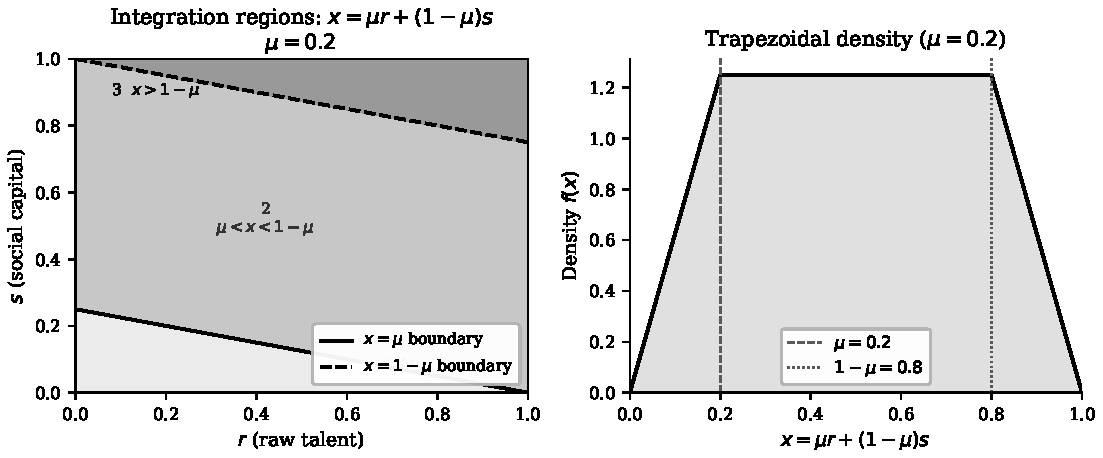
\includegraphics[width=\textwidth]{density_appendix}
\par\end{centering}
\caption{\label{fig:convex_combo}Left: ranges of $w$ and $x$ for convolution
of two scaled random variables. Right: trapezoidal density of $w$
as the convex combination with $\mu=\frac{1}{5}$.}
\end{figure}

\newpage
\section{Winning Probability Derivations} \label{sec:appendix_theoretical_2}

\subsection*{EP: High-income invests, low-income do not}

The low-income participant's score is $\mu r_i$ (no social capital).
She wins if $\mu r_i$ exceeds all $Q-1$ other low-income participants'
scores and the high-income participant's full composite score
$x_{\text{H}} = \mu r_{\text{H}} + (1-\mu)s_{\text{H}}$.
Since $\mu r_i < \mu$ for all $r_i \in (0,1)$ under
Assumption~\ref{assu:mu_less_than_half}, only the first piece of
$F_X$ applies:
\[
P_1(\text{win}|r_i) = r_i^{Q-1} \cdot F_X(\mu r_i)
= r_i^{Q-1} \cdot \frac{\mu r_i^2}{2(1-\mu)}
= \frac{\mu}{2(1-\mu)}\,r_i^{Q+1}
\]
Integrating over $r_i \sim \mathrm{Uniform}[0,1]$:
\[
p_1 = \int_0^1 \frac{\mu}{2(1-\mu)}\,r^{Q+1}\,dr
= \frac{\mu}{2(1-\mu)(Q+2)}
\]

\subsection*{IP: Low-income invest, high-income does not}

A given low-income participant wins if her full score
$x_i = \mu r_i + (1-\mu)s_i$ exceeds $x_k$ for all $Q-1$ other
low-income participants and exceeds $\mu r_{\text{H}}$ for the
non-investing high-income participant. The conditional probability is:
\[
P_1(\text{win}|r_i,s_i) = F_X(x_i)^{Q-1} \cdot G(x_i),
\quad G(x) = \begin{cases} x/\mu & 0 < x < \mu \\ 1 & x \geq \mu \end{cases}
\]
For $Q=1$ the double integral over the unit square yields:
\[
p_1' = \frac{6-7\mu}{6(1-\mu)} \quad (Q=1)
\]
For $Q \geq 2$, $F_X(x)^{Q-1} \cdot G(x)$ produces a rational
function of $\mu$ of degree $Q$ within each CDF region; each
specific $Q$ yields a closed form but no compact general formula
holds uniformly across all $Q$.

\subsection*{FW and FP}

When neither invests, scores are $\mu r_i$; by symmetry each of
$Q+1$ participants wins with probability $1/(Q+1)$:
\[
p_1 = \int_0^1 r^Q\,dr = \frac{1}{Q+1}
\]
When both invest, all scores $x_i$ are identically distributed via
$F_X$; by symmetry $p_1 = 1/(Q+1)$ again.

\subsection*{Integration regions}

To calculate $\int\!\!\int P(\text{win}|r,s)\,dr\,ds$
over the unit square, we split by the boundaries of the piecewise function.
The three regions are shown in Figure~\ref{fig:integral_boundaries}.
If $x=\mu r+(1-\mu)s$ and $F(x)$ is of the piecewise form with pieces $A$, $B$, $C$:

\begin{align*}
\int\!\!\int F(x)\,ds\,dr
 & =\int_{r=0}^{1}\!\int_{0}^{\frac{\mu(1-r)}{1-\mu}}\!\!A\,ds\,dr
 +\int_{r=0}^{1}\!\int_{\frac{\mu(1-r)}{1-\mu}}^{1-\frac{\mu r}{1-\mu}}\!\!B\,ds\,dr
 +\int_{r=0}^{1}\!\int_{1-\frac{\mu r}{1-\mu}}^{1}\!\!C\,ds\,dr
\end{align*}

\begin{figure}[H]
\begin{centering}
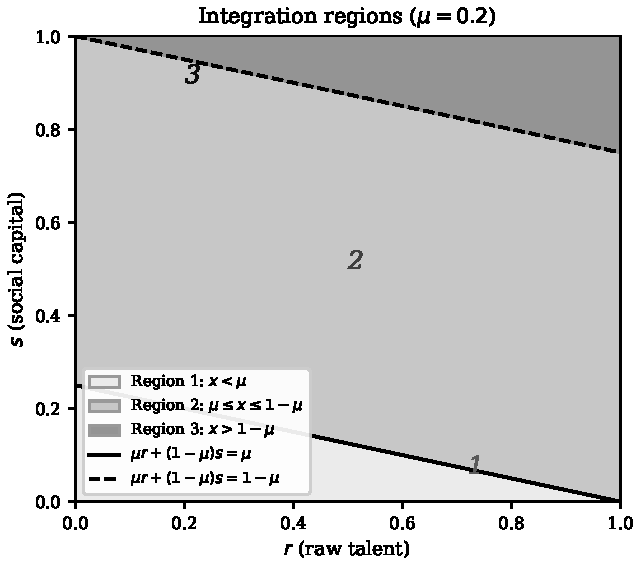
\includegraphics[width=0.85\textwidth]{integral_regions}
\par\end{centering}
\caption{\label{fig:integral_boundaries}Integration over $r,s$ split by boundaries
$\mu r+(1-\mu)s=\mu$ and $\mu r+(1-\mu)s=1-\mu$}
\end{figure}

\newpage

\subsection*{Asymptotic probability surplus}

\begin{prop}[Asymptotic probability surplus]\label{prop:asymptotic_phi}
\[
\lim_{Q \to \infty} Q(Q+1)\,\Phi(Q) = 1
\]
equivalently, $\Phi(Q) = \dfrac{1}{Q(Q+1)}\bigl[1 + O(1/Q^2)\bigr]$.
The convergence is $O(1/Q^3)$ and independent of $\mu$.
\end{prop}

\begin{proof}
Write $\Phi(Q) = \int_0^1 F_X(t)^{Q-1}[G(t)-F_X(t)]\,f_X(t)\,dt$,
where the identity follows from $p_1' = \int F_X^{Q-1}G\,f_X\,dt$
and $1/(Q+1) = \int F_X^Q\,f_X\,dt$. As $Q\to\infty$, $F_X(t)^{Q-1}$
concentrates near $t=1$. Setting $u=1-t$ and $c=\mu(1-\mu)$:
$F_X\sim 1-u^2/(2c)$, $G-F_X\sim u^2/(2c)$, $f_X\sim u/c$.
By Laplace's method:
\[
\Phi(Q) \sim \frac{1}{2c^2}\int_0^\infty u^3\exp\!\left(-\frac{Qu^2}{2c}\right)du
= \frac{1}{2c^2}\cdot\frac{2c^2}{Q^2} = \frac{1}{Q^2}
\]
Since $c=\mu(1-\mu)$ cancels, the leading term is $\mu$-independent.
The correction is $O(1/Q^3)$. $\square$
\end{proof}

\begin{corollary}\label{cor:caseII_impossible}
$Q\cdot\Phi(Q) \to 0$ at rate $1/Q$. The IP feasibility
condition $U_1 < \Phi(Q)$ fails for all $U_1 > 0$ for sufficiently
large $Q$: IP is asymptotically impossible.
\end{corollary}

\medskip\noindent
Table~\ref{tab:phi_values} reports $\Phi(Q)$ for $Q=1,\ldots,10$
at representative values of $\mu$, confirming the rapid convergence
and $\mu$-independence.

\begin{table}[H]
\centering
\caption{\label{tab:phi_values}Probability surplus $\Phi(Q)$ and
asymptotic approximation $1/[Q(Q+1)]$}
\smallskip
\begin{tabular}{rcccccc}
\toprule
$Q$ & $\mu=0.1$ & $\mu=0.2$ & $\mu=0.3$ & $\mu=0.4$
    & $1/[Q(Q\!+\!1)]$ & $Q(Q\!+\!1)\Phi$\\
\midrule
1  & 0.4815 & 0.4583 & 0.4286 & 0.3889 & 0.5000 & 0.917\\
2  & 0.1664 & 0.1651 & 0.1621 & 0.1556 & 0.1667 & 0.991\\
3  & 0.0833 & 0.0832 & 0.0829 & 0.0816 & 0.0833 & 0.998\\
4  & 0.0500 & 0.0500 & 0.0499 & 0.0497 & 0.0500 & 1.000\\
5  & 0.0333 & 0.0333 & 0.0333 & 0.0333 & 0.0333 & 1.000\\
6  & 0.0238 & 0.0238 & 0.0238 & 0.0238 & 0.0238 & 1.000\\
7  & 0.0179 & 0.0179 & 0.0179 & 0.0179 & 0.0179 & 1.000\\
8  & 0.0139 & 0.0139 & 0.0139 & 0.0139 & 0.0139 & 1.000\\
9  & 0.0111 & 0.0111 & 0.0111 & 0.0111 & 0.0111 & 1.000\\
10 & 0.0091 & 0.0091 & 0.0091 & 0.0091 & 0.0091 & 1.000\\
\bottomrule
\end{tabular}
\begin{minipage}{\textwidth}
\smallskip
{\footnotesize Values computed via numerical double integration. The
last column reports $Q(Q+1)\Phi(Q)$ at $\mu=0.2$; values at other
$\mu$ are identical to the precision shown for $Q\geq4$.}
\end{minipage}
\end{table}

\section{T-Period Utility Generalisation}\label{sec:appendix_Tperiod}

The main text presents intertemporal utility under $T$ periods with
discount sum $D_{T}=\sum_{t=0}^{T-2}\delta^{-t}$. We establish
here that the qualitative equilibrium structure is unchanged by $T$.

\medskip
\noindent\textbf{Closed form for $D_{T}$.} Since $\delta>1$, the
geometric sum evaluates to:
\[
D_{T}=\frac{1-\delta^{-(T-1)}}{1-\delta^{-1}}
\]
For $T=2$: $D_{T}=1$, recovering the two-period model. For $T=3$:
$D_{T}=1+1/\delta$.

\medskip
\noindent\textbf{Proposition (T-period invariance).} \textit{The
set of Nash equilibria under $T$-period utility is identical to
that under two-period utility ($T=2$). The participation threshold
$\overline{\nu}^{*}$ scales monotonically with $D_{T}$: it is
strictly increasing in $T$ and strictly decreasing in $\delta$.}

\medskip
\noindent\textit{Proof.} All Nash equilibrium conditions (Equations
\ref{eq:caseI_poor}--\ref{eq:caseIV_rich}) share the structure:
\[
\frac{D_{T}}{\delta}\cdot\Delta p\cdot(u(y_{2})-u(y_{1}))\gtrless U_{i}
\]
where $\Delta p$ is a probability gap and $U_{i}$ is a utility
cost. Since $D_{T}/\delta$ is a common positive scaling factor,
it does not alter which side of any inequality is larger: an equilibrium
condition satisfied under $T=2$ is satisfied for all $T\geq2$ with
the same qualitative direction. The threshold $\overline{\nu}^{*}$
(Equation~\ref{eq:nu_star}) has $A\propto D_{T}/\delta$; since
$(y_{1}/y_{2})^{A}$ is decreasing in $A$ and $y_{1}<y_{2}$,
$\overline{\nu}^{*}=y_{1}(1-(y_{1}/y_{2})^{A})$ increases with
$A$, hence with $D_{T}$. $D_{T}$ is strictly increasing in $T$
(adding positive terms) and strictly decreasing in $\delta$ (each
term $\delta^{-t}$ is decreasing in $\delta$). $\square$

\medskip
The proposition implies that a longer investment horizon or greater
patience raises $\overline{\nu}^{*}$, expanding the range of costs
under which universal participation (FP) is sustained. The
two-period model is therefore a conservative baseline: all comparative
statics on $\overline{\nu}^{*}$ with respect to $\mu$ and $Q$
carry over unchanged to the $T$-period case.


\subsection*{Log utility closed form}

Under log utility $u(y)=\log(y)$, the participation threshold
$\overline{\nu}^{*}$ has a tractable closed form. The indifference
condition $U_{1}=\frac{D_{T}}{\delta}\left(\frac{1}{Q+1}-p_{1}\right)(u(y_{2})-u(y_{1}))$
becomes:
\begin{align}
\log\frac{y_{1}}{y_{1}-\overline{\nu}^{*}} & =A\log\frac{y_{2}}{y_{1}}
\end{align}
where $A=\frac{D_{T}}{\delta}\left(\frac{1}{Q+1}-\frac{\mu}{2(1-\mu)(Q+2)}\right)>0$.
Solving:
\begin{align}
\overline{\nu}^{*} & =y_{1}\left(1-\left(\frac{y_{1}}{y_{2}}\right)^{A}\right)\label{eq:nu_star}
\end{align}

Since $(y_{1}/y_{2})^{A}$ is decreasing in $A$ and $y_{1}<y_{2}$,
$\overline{\nu}^{*}$ is increasing in $A$, hence decreasing in $\mu$
and $Q$ (since $\partial A/\partial\mu<0$ and $\partial A/\partial Q<0$).
The threshold depends on the income ratio $y_{1}/y_{2}$ rather than
the income level alone.

\section{Utility Payoffs} \label{sec:appendix_payoffs}

Table~\ref{tab:prisoners_dilemma} reports the full utility payoffs
for each of the four investment cases. In each cell, the upper entry
is the high-income participant's utility and the lower entry is the
low-income participant's utility. The scale factor $D_{T}/\delta$
multiplies all second-period terms.


\begin{table}[H]
\centering
\caption{\label{tab:prisoners_dilemma}Utility payoffs (scale factor $D_{T}/\delta$
multiplies all second-period terms)}
\smallskip
\resizebox{\textwidth}{!}{%
\begin{tabular}{llcc}
\toprule
 & & \textit{Low-income withdraws} & \textit{Low-income invests}\\
\midrule
\addlinespace[3pt]
\multirow{2}{*}{\textit{\shortstack[l]{High-income\\withdraws}}}
 & High-income
 & $u(y_{2})+\frac{D_{T}}{\delta}\!\left[\frac{u(y_{2})}{Q+1}+\frac{Qu(y_{1})}{Q+1}\right]$
 & $u(y_{2})+\frac{D_{T}}{\delta}\!\left[(1-Qp_{1}')u(y_{2})+Qp_{1}'u(y_{1})\right]$
 \\[10pt]
 & Low-income
 & $u(y_{1})+\frac{D_{T}}{\delta}\!\left[\frac{u(y_{2})}{Q+1}+\frac{Qu(y_{1})}{Q+1}\right]$
 & $u(y_{1}-\overline{\nu})+\frac{D_{T}}{\delta}\!\left[p_{1}'u(y_{2})+(1-p_{1}')u(y_{1})\right]$
 \\[6pt]
\addlinespace[3pt]
\midrule
\addlinespace[3pt]
\multirow{2}{*}{\textit{\shortstack[l]{High-income\\invests}}}
 & High-income
 & $u(y_{2}-\overline{\nu})+\frac{D_{T}}{\delta}\!\left[p_{2}u(y_{2})+(1-p_{2})u(y_{1})\right]$
 & $u(y_{2}-\overline{\nu})+\frac{D_{T}}{\delta}\!\left[\frac{u(y_{2})}{Q+1}+\frac{Qu(y_{1})}{Q+1}\right]$
 \\[10pt]
 & Low-income
 & $u(y_{1})+\frac{D_{T}}{\delta}\!\left[p_{1}u(y_{2})+(1-p_{1})u(y_{1})\right]$
 & $u(y_{1}-\overline{\nu})+\frac{D_{T}}{\delta}\!\left[\frac{u(y_{2})}{Q+1}+\frac{Qu(y_{1})}{Q+1}\right]$
 \\[6pt]
\addlinespace[3pt]
\bottomrule
\end{tabular}}
\begin{minipage}{\textwidth}
\smallskip
{\footnotesize $p_{1},p_{2}$: EP probabilities. $p_{1}'$: IP low-income probability
($Q=1$ closed form; general $Q$ numerical). The high-income participant's IP
probability satisfies $1-Qp_{1}'$, using the identity
$1/(Q+1)-(1-Qp_{1}')=Q(p_{1}'-1/(Q+1))$, valid for all $Q\geq1$.}
\end{minipage}
\end{table}



\bigskip
\noindent\textit{Corresponding author:} Anurag Srivastava, Riskcare Ltd., anurag.srivastava@riskcare.com. ORCiD: 0000-0002-6477-4430.

\end{document}
